%%%%%%%%%%%%%%%%%%%%%%%%%%%%%%%%%%%%%%%%%
% Short Sectioned Assignment LaTeX Template Version 1.0 (5/5/12)
% This template has been downloaded from: http://www.LaTeXTemplates.com
% Original author:  Frits Wenneker (http://www.howtotex.com)
% License: CC BY-NC-SA 3.0 (http://creativecommons.org/licenses/by-nc-sa/3.0/)
%%%%%%%%%%%%%%%%%%%%%%%%%%%%%%%%%%%%%%%%%

%----------------------------------------------------------------------------------------
%	PACKAGES AND OTHER DOCUMENT CONFIGURATIONS
%----------------------------------------------------------------------------------------

\documentclass[paper=a4, fontsize=11pt]{scrartcl} % A4 paper and 11pt font size

% ---- Entrada y salida de texto -----

%\usepackage[T1]{fontenc} % Use 8-bit encoding that has 256 glyphs
\usepackage[utf8]{inputenc}

\usepackage{mathptmx}
\usepackage{fourier}  % Use the Adobe Utopia font for the document - comment this line to return to the LaTeX default

% ---- Idioma --------

\usepackage[spanish, es-tabla]{babel} % Selecciona el español para palabras introducidas automáticamente, p.ej. "septiembre" en la fecha y especifica que se use la palabra Tabla en vez de Cuadro

% ---- Otros paquetes ----

\usepackage{url} % ,href} %para incluir URLs e hipervínculos dentro del texto (aunque hay que instalar href)
\usepackage{amsmath,amsfonts,amsthm} % Math packages
%\usepackage{graphics,graphicx, floatrow} %para incluir imágenes y notas en las imágenes
\usepackage{graphics,graphicx, float} %para incluir imágenes y colocarlas
\graphicspath{ {images/} }
\usepackage{subfig}

\usepackage{algorithm}
\usepackage{algpseudocode}

\usepackage{wrapfig}

% Para hacer tablas comlejas
\usepackage{multirow}
%\usepackage{threeparttable}

%\usepackage{sectsty} % Allows customizing section commands
%\allsectionsfont{\centering \normalfont\scshape} % Make all sections centered, the default font and small caps

\usepackage{fancyhdr} % Custom headers and footers
\pagestyle{fancyplain} % Makes all pages in the document conform to the custom headers and footers
\fancyhead{} % No page header - if you want one, create it in the same way as the footers below
\fancyfoot[L]{} % Empty left footer
\fancyfoot[C]{} % Empty center footer
\fancyfoot[R]{\thepage} % Page numbering for right footer
\renewcommand{\headrulewidth}{0pt} % Remove header underlines
\renewcommand{\footrulewidth}{0pt} % Remove footer underlines
\setlength{\headheight}{13.6pt} % Customize the height of the header

\numberwithin{equation}{section} % Number equations within sections (i.e. 1.1, 1.2, 2.1, 2.2 instead of 1, 2, 3, 4)
\numberwithin{figure}{section} % Number figures within sections (i.e. 1.1, 1.2, 2.1, 2.2 instead of 1, 2, 3, 4)
\numberwithin{table}{section} % Number tables within sections (i.e. 1.1, 1.2, 2.1, 2.2 instead of 1, 2, 3, 4)

\setlength\parindent{0pt} % Removes all indentation from paragraphs - comment this line for an assignment with lots of text

\newcommand{\horrule}[1]{\rule{\linewidth}{#1}} % Create horizontal rule command with 1 argument of height


\everymath{\displaystyle}
%----------------------------------------------------------------------------------------
%	TÍTULO Y DATOS DEL ALUMNO
%----------------------------------------------------------------------------------------

\title{	
\normalfont \normalsize 
\textsc{\textbf{Metaheurística} \\ Grado en Ingeniería Informática \\ Universidad de Granada} \\ [25pt] % Your university, school and/or department name(s)
\horrule{0.5pt} \\[0.4cm] % Thin top horizontal rule
\huge Práctica 1.a Técnicas de Búsqueda Local y Algoritmos Greedy para el Problema de la Mínima Dispersión Diferencial \\ % The assignment title
\horrule{2pt} \\[0.5cm] % Thick bottom horizontal rule
}

\author{José Luis Molina Aguilar} % Nombre y apellidos

\date{\normalsize\today} % Incluye la fecha actual


%----------------------------------------------------------------------------------------
% DOCUMENTO
%----------------------------------------------------------------------------------------

\begin{document}


\maketitle % Muestra el Título
  \begin{large}
    \centering
  \vfill
  
  Curso 2021-2022\\
  DNI : 77556436E\\
  Correo : joselu201@correo.ugr.es\\
  Grupo : A3, MARTES 17:30 - 19:30
  \vfill
  \end{large}
\newpage %inserta un salto de página

\tableofcontents % para generar el índice de contenidos

\listoffigures


\newpage



%----------------------------------------------------------------------------------------
%	Cuestión 1
%----------------------------------------------------------------------------------------

\section{Descripción Problema de Mínima Dispersión Diferencial}
El problema de Mínima Dispersión Diferencial es un problema de optimización combinatoria que entra en la clase de problemas
\textbf{NP-Completo}\\
Este es un problema en el que las heurísticas obtienen buenas soluciones en menos tiempo.
 
\subsection{Descripción}
Dado un conjunto de $n$ elementos todos ellos conectados entre sí, representado por una matriz de distancias de tamaño $nxn$
obtener un subconjunto $m$ tal que la diferencia entre la máxima distancia acumulada y la mínima distancia acumulada de los elementos de $m$
se minimiza.\\
El conjunto $m < n$ y por lo tanto lo que estamos buscando es
$ m \subset n \mid Minimize DD(S_m) $\\
donde $DD(S_m) $ es la Dispersión Diferencial del conjunto de Soluciones de tamaño $m$\\
\subsection{Consideraciones}
En mi representación de este problema la matriz de distancias descrita anteriormente será una matriz de flotantes llamada \textbf{datos}\\
 
 
Además implementaré un vector \textbf{distan} la cual almacena la distancia desde un punto al resto, será útil para factorizar en BL.\\
 
\section{Greedy}
El algoritmo Greedy se basa en la heurística de ir añadiendo a la solución el elemento más óptimo de los disponibles, el cual es el que minimice la dispersión.\\
Elegiremos el primer elemento de $m$ de forma aleatoria para ganar variedad en los resultados.\newline
Después, el resto de elementos a elegir hasta completar la solución será, sobre todos los posibles candidatos,
calculamos la dispersión cuando añadimos ese elemento a la solución $m$ y
el elemento que la minimice será escogido y añadido a la solución.\\
Esta aproximación cae fácilmente en óptimos locales ya que es muy dependiente de los del punto de inicio y en cada paso aunque escojamos
el elemento que minimiza la Dispersión no significa que, como conjunto solución, sea el correcto.\\
La ventaja principal del greedy es que obtiene una solución relativamente buena en mucho menos tiempo que el algoritmo perfecto que resuelve este problema.
 
Para ayudarnos en el desarrollo del Greedy usaremos 3 funciones:\\

\begin{itemize}
  \item \textbf{distPuntoRestoElemenetos}, que calcula la distancia acumulada de un punto al resto del vector.
  \item\textbf{diff}, el cual dado un vector de soluciones calcule las distancias acumuladas (distPuntoRestoElemenetos)
  y devuelva la dispersión para ese conjunto.\\
  \item \textbf{fit\_adding}, esta función simplemente calcula la dispersión (mediante diff) si añadimos un nuevo elemento al vector de soluciones.
\end{itemize}

 
La representación de la solución la realizaremos con un vector de enteros que almacena los índices de los elementos escogidos.
 
Por lo que el algoritmo Greedy quedaría:\\
\begin{algorithm}[H]
  \caption{Greedy}
  \label{Greedy}
  \begin{algorithmic}[1]
    \Function{Greedy}{}
      \State $Solucion \gets \emptyset$
      \State $Candidatos \gets V$ \Comment{V son todos los indices, $n$}
      \State $v_0 \gets SelectRandomFrom(Candidatos)$
      \State $Solucion \gets Solucion \cup  \{v_0\}$
      \State $Candidatos \gets Candidatos \setminus  \{v_0\}$
      \While{$|Solucion| < m $}
        \For{ele in Candidatos}
          \State $min \gets FLOATMAX$
          \State $new\_fitness \gets \texttt{fit\_adding(Solucion, ele)}$
          \If{$new\_fitness < min$ }
            \State $ele\_pos \gets ele$ \Comment{Guardo el mejor elemento}
            \State $min \gets new\_fitness$ \Comment{Actualizo el minimo actual}
          \EndIf
        \EndFor
        \State $Solucion \gets Solucion \cup \{ele\_pos\}$  \Comment{Añado a la solucion}
        \State $Candidatos \gets Candidatos \setminus  \{ele\_pos\}$

      \EndWhile
      \label{euclidendwhile}
      \State \Return{$Solucion$}
    \EndFunction
  \end{algorithmic}
\end{algorithm}
\newpage
Pseudocodigo de \textbf{distPuntoRestoElemenetos}
\begin{algorithm}[H]
  \caption{distPuntoRestoElemenetos}
  \begin{algorithmic}[1]
    \Function{distPuntoRestoElemenetos(fila,vector)}{}
      \State $dist \gets 0$
        \For{$i \gets 0$ to ${length(vector)}$}
          \State $dist \gets dist + datos[fila][vector[i]]$
        \EndFor
      \label{euclidendwhile}
      \State \Return{$dist$}
    \EndFunction
  \end{algorithmic}
\end{algorithm}

Pseudocodigo de \textbf{diff}
\begin{algorithm}[H]
  \caption{diff}
  \begin{algorithmic}[1]
    \Function{diff(posibles)}{}
      \State $distancias \gets \emptyset$
      \For{$i \gets 0$ to ${length(posibles)}$}
        \State $distancias \gets distancias \cup distPuntoRestoElemenetos(posibles[i],posib))$
      \EndFor
      \State $sort(distancias)$
      \State \Return{$distancias[{length(posibles)}] - distancias[0] $}
    \EndFunction
  \end{algorithmic}
\end{algorithm}

Pseudocodigo de \textbf{fit\_adding}

\begin{algorithm}[H]
  \caption{fit\_adding}
  \begin{algorithmic}[1]
    \Function{$fit\_adding(posibles, new_i)$}{}
      \State $posibles \gets posibles \cup new_i$
      \State $new\_diff \gets \texttt{diff(posibles)}$
      \State $posibles \gets posibles \setminus new_i$
      \State \Return{$new\_diff$}
    \EndFunction
  \end{algorithmic}
\end{algorithm}


\section{Busqueda por Trayectorias Simples (BL)}
La búsqueda local se basa en generar una solución aleatoria, la cual como solución válida tiene que satisfacer las restricciones de
\begin{itemize}
  \item No puede tener elementos repetidos
  \item Tiene que tener exactamente $m $ elementos
  \item El orden no es relevante
\end{itemize}
Para obtener una solución BL aplica un Operador de intercambio, este es:\\
Dada una solución, intercambiar un elemento de esa solución por otro elemento del conjunto Candidatos, (el cual
esto formado por todos los índices menos los que están en solución, S-Solucion = Candidatos), el cual minimice el valor del fitness.\\
Esto provoca que el espacio de posibilidades de cambio sea de  $m\cdot (m-n)$, por lo que a la hora de aplicar esto, una vez que
encontremos un elemento que minimice la dispersión se añadirá a la solución, (con añadir me refiero a intercambiar los valores) y
seguidamente buscaremos otra vez para el siguiente elemento de la solución, puede llegar un punto en el que una vez recorrido
todo el conjunto de soluciones e intentar intercambiarlo por algún elemento del conjunto de Candidatos ninguno minimice el valor
actual, en ese caso terminaremos y devolveremos la solución actual.\\
También utilizaremos un número limitado de iteraciones.
 
\subsection{Factorización del Movimiento de Intercambio}
Ejemplo.\\
Dado el conjunto solución (0,4,6), cambio el elemento 0 por 1, quedaria (1,4,6) por lo que el vector distan quedaría:\\
D0 = D04 + D06  //Esta ya no lo necesito\\
D4 = D40 + D46  //Si cambio el 0 por un 1, D4 = D4 -D04 + D14\\
D6 = D60 + D64\\
------------------------------------------------------------\\
D1 = D14 + D16 //Este tengo que recalcularlo entero\\
D4 = D4 -D04 + D14\\
D6 = D6 -D06 + D16\\
 
De esta forma no tengo que volver a calcular de nuevo todas las distancia de un punto al resto,
sino que simplemente tendré que actualizar el valor de la forma anteriormente descrita.\\
Lo cual me hace pasar de una complejidad $\mathcal{O}(n^2)$ a $\mathcal{O}(n)$

\begin{algorithm}[H]
  \caption{BL}
  \label{Greedy}
  \begin{algorithmic}[1]
    \Function{BL}{}
      \State $Solucion \gets \texttt{SelectRandomSolution}$
      \State $Candidatos \gets V$ \Comment{V son todos los indices de $n$}
      \State $\texttt{Shuffle(Candidatos)}$
      \State $index \gets 0$ \Comment{Indice de solucion}
      \State $MaxIters \gets 1000000$
      \State $cambia \gets true$
      \State $iter \gets 0$
      \While{$iter < MaxIters $ and $cambia$}
        \For{$i \gets 0$ to ${length(candidatos)}$}
          \State $actual\_disp \gets \texttt{diff(Solucion)}$
          \State $intercambio \gets ( index , cand[i])$ \Comment{Cambio el elemento $index$ por un candidato}
          \State $new\_disp \gets \texttt{distFactorizada(Solucion, intercambio)}$
          \If{$new\_disp < actual_disp$ }
            \State $Solucion \gets Solucion \cup \{cand[i]\}$  \Comment{Añado a la solucion}
            \State $index \gets index +1$ \Comment{Avanzo a otro elemento de solucion}
            \State $cambio \gets true$ \Comment{Anoto que ha habido cambio}
            \State $i \gets 0$ \Comment{Vuelvo a mirar con el siguiente elemento}
          \EndIf

          \If{$!cambio$ and solucion[index] != solucion[solucion.size()]}\\
          \Comment{Si no ha habido cambio, pero no he he comprobado todo Solucion}
            \State $index \gets index +1$ \Comment{Avanzo al siguiente elemento}
            \State $i \gets 0$ \Comment{Vuelvo a mirar si algun candidato mejora}
          \ElsIf{solucion[index] == solucion[solucion.size()]} \\
          \Comment{Si he comprobado todas}
            \State $cambio \gets false$
          \EndIf
          \State $iter \gets iter +1$
        \EndFor
        \State $index \gets index +1$
      \EndWhile
      \State \Return{$Solucion$}
    \EndFunction
  \end{algorithmic}
\end{algorithm}

Pseudocodigo de \textbf{distFactorizada}
\begin{algorithm}[H]
  \begin{algorithmic}[1]
    \Function{$distFactorizada(solucion, cambio)$}{}
      \State $distan[cambio.first] = distPuntoRestoElemenetos(cambio.second,solucion);$\Comment{Recalculo el punto que he cambiado}
      \For{$i \gets 0$ to $length(solucion)$}
        \State $distan[i] \gets distan[i] - datos[solucion[cambio.first]][solucion[i]] + datos[cambio.second][solucion[i]];$
      \EndFor
      \State $\texttt{Sort(distan)}$
        \State \Return{$(distan[distan.size()-1] - distan[0] );$}
    \EndFunction
  \end{algorithmic}
\end{algorithm}

\section{Analisis}
\begin{itemize}
  \item La información de uso se encuentra en el README.md.
  \item Las semillas con las que se han obtenido los resultados entan el main.cpp y son \{0,1,2,3,4\}.
\end{itemize}

Finalmente para representar los resultados obtenidos por estos dos algoritmos respecto del perfecto tenemos la siguinte grafica
\begin{figure}[h]
  \centering
  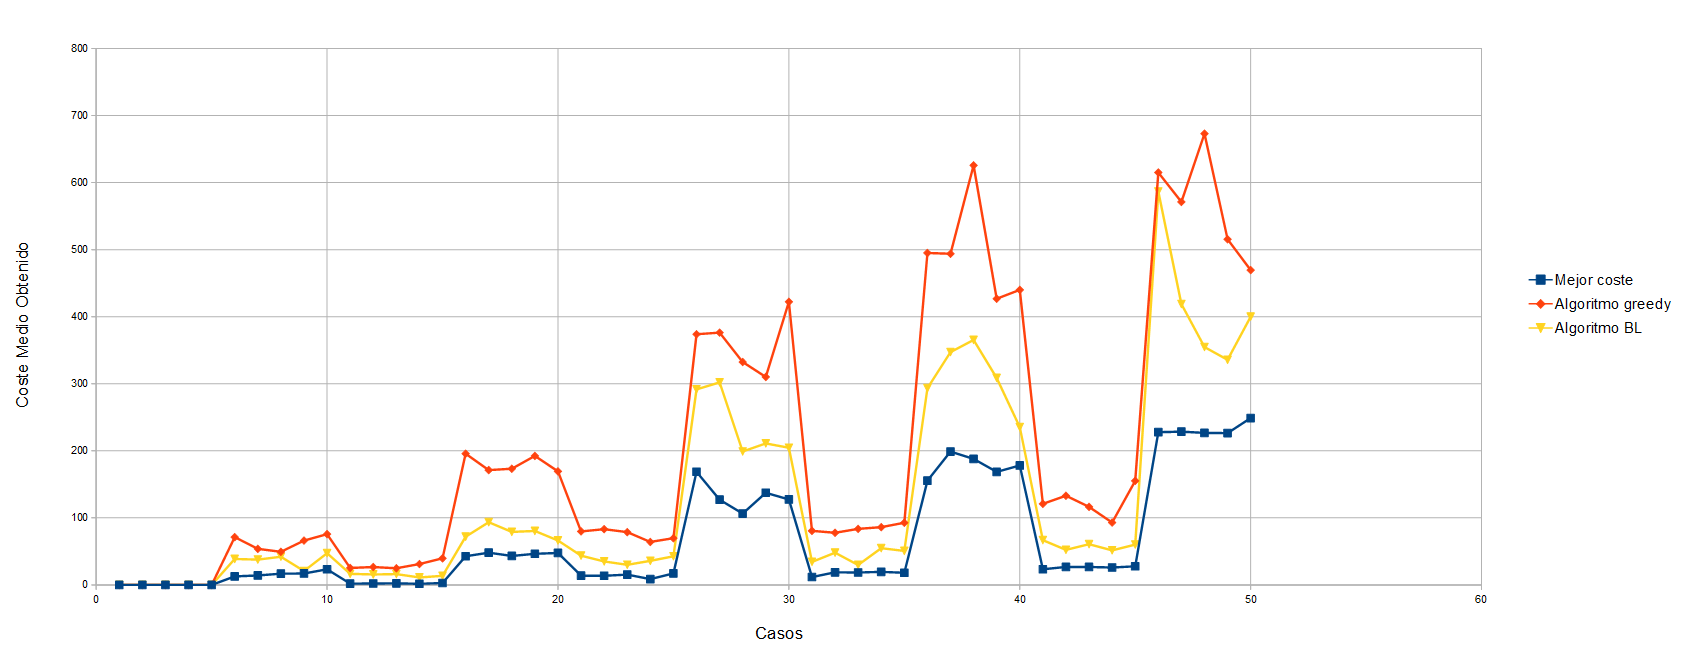
\includegraphics[width=\textwidth]{graf1}
  \caption{Resultados distintos Algoritmos}
  \label{gra}
\end{figure}


En la Gráfica \ref{gra} podemos ver como se comporta cada algoritmo, como vemos la BL es mucho mejor que el Greedy en este caso ya que 
esta mas cerca del resultado que nos ofrece el algoritmo perfecto.\newpage


\begin{figure}[h]
  \centering
  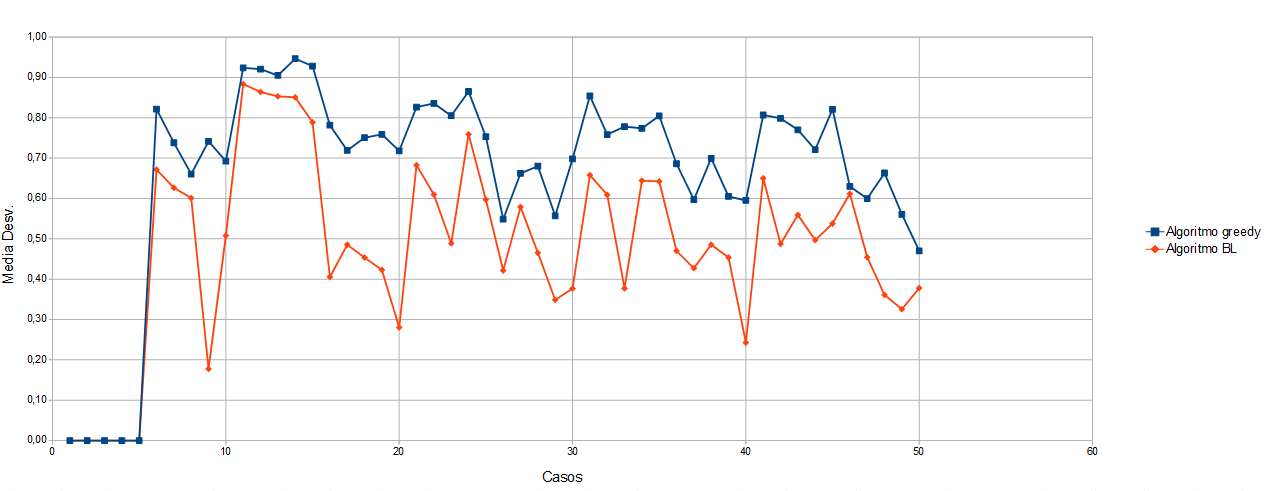
\includegraphics[width=\textwidth]{desv}
  \caption{Desviación distintos Algoritmos}
  \label{gra2}
\end{figure}

Pero esta mejora en la precisión conlleva como podemos ver el la Gráfica \ref{gra3} un aumento sustancial en el tiempo de computo
aunque si pudiesemos comparar el tiempo que le tomo al algoritmo perfecto, la BL en comparación sería muy rapida.

Además podemos ver que que el tiempo que tarda en dar una solucion es directamente proporcional al numero de elementos de $m$ ya
que, como podemos ver podemos diferenciar intervalos que tienen en comun una cosa $n$, por ejemplo [31,40 ], $n = 125$, dentro de ese
intervalo tenemos que [31-35] $m =12 $ y [35 - 40] $m =37 $, en la Gráfica podemos ver que tarda mucho menos en [31-35]
ya que el valor de $m$ es menor que en el intervalo [35 - 40]

\begin{figure}[h]
  \centering
  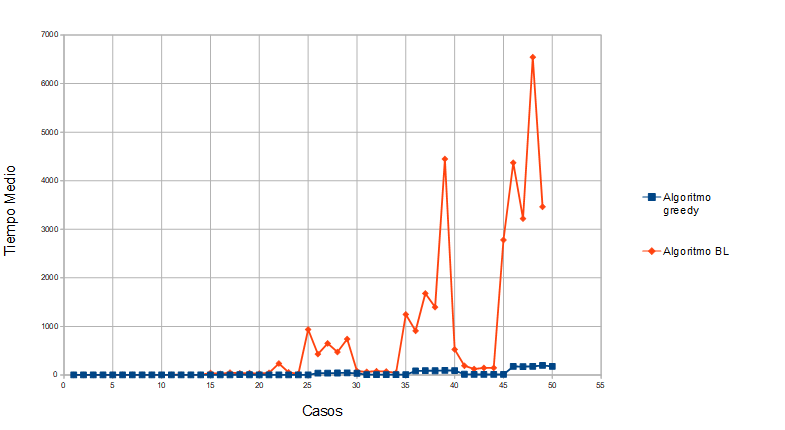
\includegraphics[width=0.9\textwidth]{tiempos}
  \caption{Tiempos(ms) para diferentes Algoritmos}
  \label{gra3}
\end{figure}

%%%%%%%%%%%%%%%%%%%%%%%%%%%%%%%%%%%%%%%%%%%%%%%%%%%%%%%%%%%%%%%%
%%%%%%%%%%%%%%%%%%%%%%%%%%%%%%%%%%%%%%%%%%%%%%%%%%%%%%%%%%%%%%%%
%%%%%%%%%%%%%%%%%%%%%%%%%%%%%%%%%%%%%%%%%%%%%%%%%%%%%%%%%%%%%%%%
%%%%%%%%%%%%%%%%%%%%%%%%%%%%%%%%%%%%%%%%%%%%%%%%%%%%%%%%%%%%%%%%


\section{P2 : Basados en Poblaciones}
En esta practica tendremos que cambiar la representacion de las solución de enteras a binarias, por lo
que ahora tendremos que cada solución tendrá un vector de $n$ elementos donde $m$ de esos elementos tienen que ser
obligatoriamente 1's lo que significará que esos genes estan activos.
Cambiaremos a esta representacion ya que es idone para realizar ejercicios basados en poblacion gracias a la facilidad 
de generar, cruzar y mutar individuos.\\

Nos ayudaremos de funciones para realizar estos algoritmos
\\begin{itemize}
  \item \textbf{generarPoblacion()} Esta funcion nos permite generar individuos aleatoriamente respentando las 
  restricciones que se nos proponen, si ejecutamos esta funcion $N$ veces obtendremos una poblacion de $N$ individuos.
  Una vez que tenemos una poblacion es siguiendo punto importante seria ser capaz de seleccionar individuos de la misma
   con el fin de cruzarlos y generar hijo, para ello
  \item  \textbf{seleccion(poblacion, n)} Esta funcion nos permitira elegir $n$ individuos de la poblacion.
  Una vez que tenemos a los individuos seleccionados tenemos que generar una seria de hijos de estos individuos seleccionados, para ello tenemos dos opciones
  
  \begin{itemize}
    \item  \textbf{generarHijosPosicion(padre1, padre2)} Esta funcion cruzara dos padres, mantendra los genes comunes y 
    eligira aleatoriamente el resto de ambos genes para decidir el resto de genes.\\
    De esta forma los hijos generados comparten un poco menos de informacion con los padres.
    \item  \textbf{generarHijosUniforme(padre1, padre2)} Esta función cruzamos dos padres, manteniendo los genes comunes y 
    eligiendo aleatoriamente el resto, esto puede provocar que los hijos que obtengamos no cumplan las restricciones, por lo que 
    a veces en necesario reparlos,
    \item  \textbf{repair(hijo)} La manera en la que reparamos se basa en si faltan elementos,
     añadir los que minimizen la disperion y si sobran elementos eliminar aquellos que minimizen la dispersion.  
  \end{itemize}

\end{itemize}

Pseudocodigo de \textbf{generarPoblacion}
\begin{algorithm}[H]
  \begin{algorithmic}[1]
    \Function{$generarPoblacion()$}{}
      \State $poblacion \gets \emptyset $\Comment{Creamos una poblacion vacia}
      \While{$count(poblacion,1) != m $} \Comment{El numero de 1 sea distinto de m}
        \State $idx \gets Random(0,n)$ \Comment{Obtenemos un numero de 0 a n}
        \If{$poblacion[idx] == 0$}
          \State{$poblacion[idx] = 1$}
        \Else{ continue;}
        \EndIf
      \EndWhile
      \State \Return{$poblacion$}
    \EndFunction
  \end{algorithmic}
\end{algorithm}

Entonces a la hora de crear una poblacion ejecutaremos esta funcion tantas veces como individuos queramos, para después
guardarlo en una matriz de todos los individuos llamada poblacion.
Ademas tendremos un vector llamadao \textbf{fitness\_i} en la cual guardaremos el fitness de cada individuo.\\

Pseudocodigo de \textbf{torneo(poblacion,fitness\_i, indiv)}
\begin{algorithm}[H]
  \begin{algorithmic}[1]
    \Function{$torneo(poblacion,fitness\_i, indiv)$}{}
      \State $torneo \gets \emptyset $\Comment{Creamos un torneo vacia}
      \State $worst \gets \infty$
      \While{$|torneo| != indiv $} \Comment{Tenemos indiv diferentes }
        \State $torneo \gets torneo \cup Random(0,|poblacion|)$ \Comment{Obtenemos un numero de 0 a n}

      \EndWhile
      \For{$i$ in $torneo$}
        \If{$fitness\_i[i] < worst$}
          \State $worst \gets fitness\_i[i] $
          \State $winner \gets i$
        \EndIf
      \EndFor
      \State \Return{$winner$}
    \EndFunction
  \end{algorithmic}
\end{algorithm}

Funcion que escoge n elementos ganadores del torneo.\\
Pseudocodigo de \textbf{seleccion(poblacion,fitness\_i, indiv,n)}
\begin{algorithm}[H]
  \begin{algorithmic}[1]
    \Function{$seleccion(poblacion,fitness\_i, indiv,n)$}{}
      \State $winner \gets \emptyset $
      \For{$i$ in $n$}
          \State $winner \gets winner \cup torneo(poblacion,fitness\_i,n)$
      \EndFor
      \State \Return{$winner$}
    \EndFunction
  \end{algorithmic}
\end{algorithm}


Pseudocodigo de \textbf{generarHijosUniforme(padre1,padre2)}
\begin{algorithm}[H]
  \begin{algorithmic}[1]
    \Function{$generarHijosUniforme(padre1,padre2)$}{}
      \State $hijos \gets \emptyset$
      \For{$i = 0 in |padre|$}
      \If{$padre1[i] == padre2[i]$}
          \State $hijos[i] \gets padre1[i]$
      \Else
          \State $hijos[i] \gets Random(0,1)$
      \EndIf
      \EndFor
      \State $reparar(hijos)$
      \State \Return{$hijos$}
    \EndFunction
  \end{algorithmic}
\end{algorithm}

Esta funcion repara la generacionde hijos cuando se generar de forma uniforme creando lo mejores hijos manteniendo 
los genes de los padres.\\

Pseudocodigo de \textbf{reparar(hijo)}
\begin{algorithm}[H]
  \begin{algorithmic}[1]
    \Function{$reparar(hijo)$}{}
      \State $v \gets count(hijos,1)$
      
      \If{$v == m $}
        \State \Return{$hijo$}
      \ElsIf{$v > m $} \Comment{Si te sobran elementos}
        \While{$v $ !=$  m $}
          \State escoger los genes que minimizan la dispersion
        \EndWhile
      \ElsIf{$v < m $} \Comment{Si te faltan elementos}
        \While{$v $ != $ m $}
          \State escoger los genes que minimizan la dispersion
        \EndWhile
      \EndIf

      \State \Return{$hijo$}
    \EndFunction
  \end{algorithmic}
\end{algorithm}

Funcion que genera una pareja de hijos que mantiene la posicoon de los genes de los padres y los que no coinciden
se selecionan aleatoriamente pero respetando las restricciones.\\
Pseudocodigo de \textbf{generarHijosPosicion(padre1,padre2)}
\begin{algorithm}[H]
  \begin{algorithmic}[1]
    \Function{$generarHijosPosicion(padre1,padre2)$}{}
      \State $hijos \gets \emptyset$
      \State $restos \gets \emptyset$

      \If{$padre1 == padre2$}
        \State $hijos = padre1,padre2$  \Comment{Devolvemos los mismos padres}
      \EndIf

      \For{$i = 0 in |padre|$}
        \If{$padre1[i] != padre2[i]$}
          \If{$padre1[i] == 0 $ and $ padre2[i] == 1 $}
            \State $resto \gets resto \cup 0$
          \ElsIf{$padre1[i] == 1$ and $ padre2[i] == 0 $}
            \State $resto \gets resto \cup 1$
          \EndIf
        \Else
          \State$continue$
        \EndIf
      \EndFor
      \State $shuffle(resto)$
      \State $j \gets 0$
      \For{$i = 0 in |padre|$}
        \If{$padre1[i] == padre2[i]$}
            \State $hijos[i] \gets padre1[i] $
        \Else
            \State $hijos[i] \gets resto[j] $
            \State $j \gets j +1$
        \EndIf
      \EndFor

      \State \Return{$hijos$}
    \EndFunction
  \end{algorithmic}
\end{algorithm}


Algoritmos geneticos:\\
Implentaremos 2 tipos de algorimos geneticos,\\
AGG( algorimo genetico generacional )\\
AGG se basa en un algorimo que genera una poblacion aleatoria,despues se escogen mediante un torneo binario tantos individuos como
poblacion del mismo y se cruzan, en nuestro caso diferenciaremos dos tipos de cruze uniforme y posicion (cuyos Pseudocodigo estas explicado arriba)
para seguidamente mutar algunos de sus genes con probabilidad $P_M$ y reemplazar la nueva poblacion obtenida por la nueva y conservando el mejor de ambas(elitismo).\\
AGE( algorimo genetico Estacional )\\  
Este es practicamente igual, la unica diferencia es que a laa hora de selecionar los individuos, solo se seleccionan 2, estos seran los que se cruzaran y cuyos hijos mutaran, 
para seguidamente, si mejoran los peores individuos de la poblacion sustituirlos.



\begin{algorithm}[H]
  \begin{algorithmic}[1]
    \Function{$AGG\_uniforme()$}{}
      \State $TAM = 50$
      \State $MAX\_ITERS = 100000$
      \State $iters = 0$

      \State $poblacion \gets \emptyset$ \Comment{Matriz de TAM individuos}
      \State $hijo \gets \emptyset$ \Comment{Este sera el hijo solucion}
      \State $hijos \gets \emptyset$
      \State $fitness\_i \gets \emptyset$
      
      \For{$row $ in $poblacion$}
        \State $row \gets generarPoblacion()$
        \State $fitness\_i \gets fitness\_i \cup diff(row)$
      \EndFor

      \While{$iters < MAX\_ITERS$}
        \State $best\_father \gets  best(poblacion)$ \Comment{Individuo de la poblacion con la menor dispersión}

        \For{$row$ in $|poblacion|$}
          \State $padre2 \gets next(row)$ \Comment{Siguiente individuo}
          \If{$bool Random(0.7)$}
            \State $hijos \gets hijos \cup generarHijosUniforme(row,padre2)$
            \State $fitness\_i \gets fitness\_i \cup diff(hijos)$  \Comment{Actualizamos la dispersion de los nuevos hijos}
          \Else
            \State $hijos \gets hijos \cup row$
          \EndIf
        \EndFor
        \State $spected\_mutations \gets 0.1*n*m$
        \State $count = 0$
        \While{$count != spected\_mutations$}
          \State $cromosoma \gets Random(0,TAM)$ \Comment{Elegimos el Individuo a mutar}
          \State $gen1 \gets Random(0,n)$
          \State $gen2 \gets Random(0,n)$ \Comment{Elegimos dos genes Diferentes}

          \If{$hijos at cromosoma[gen1] !=  hijos at cromosoma[gen2]$} \Comment{Si los genes del individuos elegido en hijos son distintos}
            \State $swap(hijos at cromosoma[gen1], hijos at cromosoma[gen2])$
          \EndIf
          \State $count \gets count +1 $
        \EndWhile

        \State $poblacion \gets hijos$ \Comment{Los hijos sustituyen a la poblacion actual}

        \If{$!find(fitness\_i, best\_father)$} \Comment{Si no encuentro el mejor individuo de la poblacion  sustituyo el peor por el mejor de la anterior}
          \State $poblacion at peor elemento \gets best\_father$
        \EndIf
      \EndWhile

      \State $hijo \gets min(poblacion)$
      
      \State \Return{$hijo$}
    \EndFunction
  \end{algorithmic}
\end{algorithm}

\begin{algorithm}[H]
  \begin{algorithmic}[1]
    \Function{$AGG\_posicion()$}{}
      \State $TAM = 50$
      \State $MAX\_ITERS = 100000$
      \State $iters = 0$

      \State $poblacion \gets \emptyset$ \Comment{Matriz de TAM individuos}
      \State $hijo \gets \emptyset$ \Comment{Este sera el hijo solucion}
      \State $hijos \gets \emptyset$
      \State $fitness\_i \gets \emptyset$
      
      \For{$row $ in $poblacion$}
        \State $row \gets generarPoblacion()$
        \State $fitness\_i \gets fitness\_i \cup diff(row)$
      \EndFor

      \While{$iters < MAX\_ITERS$}
        \State $best\_father \gets  best(poblacion)$ \Comment{Individuo de la poblacion con la menor dispersión}

        \For{$row$ in $|poblacion|$}
          \State $padre2 \gets next(row)$ \Comment{Siguiente individuo}
          \If{$bool Random(0.7)$}
            \State $hijos \gets hijos \cup generarHijosPosicion(row,padre2)$
            \State $fitness\_i \gets fitness\_i \cup diff(hijos)$  \Comment{Actualizamos la dispersion de los nuevos hijos}
          \Else
            \State $hijos \gets hijos \cup row$
          \EndIf
        \EndFor
        \State $spected\_mutations \gets 0.1*n*m$
        \State $count = 0$
        \While{$count != spected\_mutations$}
          \State $cromosoma \gets Random(0,TAM)$ \Comment{Elegimos el Individuo a mutar}
          \State $gen1 \gets Random(0,n)$
          \State $gen2 \gets Random(0,n)$ \Comment{Elegimos dos genes Diferentes}

          \If{$hijos at cromosoma[gen1] !=  hijos at cromosoma[gen2]$} \Comment{Si los genes del individuos elegido en hijos son distintos}
            \State $swap(hijos at cromosoma[gen1], hijos at cromosoma[gen2])$
          \EndIf
          \State $count \gets count +1 $
        \EndWhile

        \State $poblacion \gets hijos$ \Comment{Los hijos sustituyen a la poblacion actual}

        \If{$!find(fitness\_i, best\_father)$} \Comment{Si no encuentro el mejor individuo de la poblacion  sustituyo el peor por el mejor de la anterior}
          \State $poblacion at peor elemento \gets best\_father$
        \EndIf
      \EndWhile

      \State $hijo \gets min(poblacion)$
      
      \State \Return{$hijo$}
    \EndFunction
  \end{algorithmic}
\end{algorithm}



\begin{algorithm}[H]
  \begin{algorithmic}[1]
    \Function{$AGE\_uniforme()$}{}
      \State $TAM = 50$
      \State $MAX\_ITERS = 100000$
      \State $iters = 0$

      \State $poblacion \gets \emptyset$ \Comment{Matriz de TAM individuos}
      \State $hijo \gets \emptyset$ \Comment{Este sera el hijo solucion}
      \State $hijos \gets \emptyset$
      \State $fitness\_i \gets \emptyset$
      \State $fitness\_hijo \gets \emptyset$
      
      \For{$row $ in $poblacion$}
        \State $row \gets generarPoblacion()$
        \State $fitness\_i \gets fitness\_i \cup diff(row)$
      \EndFor

      \While{$iters < MAX\_ITERS$}
        
        \State $selected \gets seleccion(poblacion,fitness\_i,2)$\Comment{Eligo los 2 padres}
        \State $hijos \gets generarHijosUniforme(selected[0],selected[1])$\Comment{Cruzo los 2 padres}
        
        \State $spected\_mutations \gets 0.1*n*2$
        \State $count = 0$
        \While{$count != spected\_mutations$}
          \State $cromosoma \gets Random(0,|hijos|)$ \Comment{Elegimos el Individuo a mutar}
          \State $gen1 \gets Random(0,n)$
          \State $gen2 \gets Random(0,n)$ \Comment{Elegimos dos genes Diferentes}

          \If{$hijos at cromosoma[gen1] !=  hijos at cromosoma[gen2]$} \Comment{Si los genes del individuos elegido en hijos son distintos}
            \State $swap(hijos at cromosoma[gen1], hijos at cromosoma[gen2])$ \Comment{Intercambio cromosomas}
            \State $fitness\_hijo \gets fitness\_hijo \cup hijos at cromosoma$ \Comment{Actualizo dispersion}
          \EndIf
          \State $count \gets count +1 $
        \EndWhile

        \State $worst\_i,second\_worst \gets max(fitness\_i)$ \Comment{Obtengo los dos peores padres}
       
        \State $poblacion \gets poblacion \cap \{worst\_i,second\_worst\}$
        \State $poblacion \gets poblacion \cup {hijos}$ \Comment{Sustituyo los peores padres por los mejores hijos}
      
      \EndWhile
      
      \State $hijo \gets min(poblacion)$
      \State \Return{$hijo$}
    \EndFunction
  \end{algorithmic}
\end{algorithm}

\begin{algorithm}[H]
  \begin{algorithmic}[1]
    \Function{$AGE\_posicion()$}{}
      \State $TAM = 50$
      \State $MAX\_ITERS = 100000$
      \State $iters = 0$

      \State $poblacion \gets \emptyset$ \Comment{Matriz de TAM individuos}
      \State $hijo \gets \emptyset$ \Comment{Este sera el hijo solucion}
      \State $hijos \gets \emptyset$
      \State $fitness\_i \gets \emptyset$
      \State $fitness\_hijo \gets \emptyset$
      
      \For{$row $ in $poblacion$}
        \State $row \gets generarPoblacion()$
        \State $fitness\_i \gets fitness\_i \cup diff(row)$
      \EndFor

      \While{$iters < MAX\_ITERS$}
        
        \State $selected \gets seleccion(poblacion,fitness\_i,2)$\Comment{Eligo los 2 padres}
        \State $hijos \gets generarHijosPosicion(selected[0],selected[1])$\Comment{Cruzo los 2 padres}
        
        \State $spected\_mutations \gets 0.1*n*2$
        \State $count = 0$
        \While{$count != spected\_mutations$}
          \State $cromosoma \gets Random(0,|hijos|)$ \Comment{Elegimos el Individuo a mutar}
          \State $gen1 \gets Random(0,n)$
          \State $gen2 \gets Random(0,n)$ \Comment{Elegimos dos genes Diferentes}

          \If{$hijos at cromosoma[gen1] !=  hijos at cromosoma[gen2]$} \Comment{Si los genes del individuos elegido en hijos son distintos}
            \State $swap(hijos at cromosoma[gen1], hijos at cromosoma[gen2])$ \Comment{Intercambio cromosomas}
            \State $fitness\_hijo \gets fitness\_hijo \cup hijos at cromosoma$ \Comment{Actualizo dispersion}
          \EndIf
          \State $count \gets count +1 $
        \EndWhile

        \State $worst\_i,second\_worst \gets max(fitness\_i)$ \Comment{Obtengo los dos peores padres}
       
        \State $poblacion \gets poblacion \cap \{worst\_i,second\_worst\}$
        \State $poblacion \gets poblacion \cup {hijos}$ \Comment{Sustituyo los peores padres por los mejores hijos}
      
      \EndWhile
      
      \State $hijo \gets min(poblacion)$
      \State \Return{$hijo$}
    \EndFunction
  \end{algorithmic}
\end{algorithm}

Algoritmo Memético
Este algoritmo consiste en hibridar el AGG con una busqueda local, sabemos que  BL obtiene buenos resultados en poco tiempo, por lo que La
idea de este algoritmo seria mejorar la poblacion mediante BL de esta forma la solucion seria bastante aproximada, pero si seguimos ejecutando cruces y mutaciones
salir del espacio de busqueda local para seguir explorando mejores soluciones.
La diferencia de entre estos tres algoritmos Memeticos será sobre que individuos aplicar la BL.
\begin{itemize}
  \item Cuando aplicamos la BL sobre toda la poblacion obtenemos muy buenas poblaciones, por lo que a la hora de seguir cruzando y mutando los individuos, como comparten genes seguiremos obtendendo buenos resultados. 
  \item Si aplicamos BL sobre un subconjunto de la poblacion mejoraremos un poco esos individuos, pero como el cruze se hace con toda la poblacion no se mejora tanto la poblacion, o en cualquir caso tardara mas iteraciones en mejorar toda la solucion
  \item En el ultimo caso solo aplicamos BL sobre los mejores individuos (0.1) esto implica que esos individuos obtienen muy buenas soluciones, pero al cruzarse con una poblacion no tan buena tienen a no ser muy buena idea, aunque igualmente obtiene buenos resultados

\end{itemize}

Cabe destavar que el algoritmo de BL usado es el mismo que el de la practica 1 excepto que en vez de generar una solucion se la pasamos como parametro,
como esa solucion que le pasamos esta en representacion binaria tenemos que transformarla a representacion entera y una vez encontrada la solucion volver a pasarla a representación binaria
Pseudocodigo de AM, el cual cada 10 iteraciones aplico BL sobre todos los elementos de la poblacion.
\begin{algorithm}[H]
  \begin{algorithmic}[1]
    \Function{$AM\_all()$}{}
      \State $TAM = 50$
      \State $MAX\_ITERS = 100000$
      \State $iters = 0$

      \State $poblacion \gets \emptyset$ \Comment{Matriz de TAM individuos}
      \State $hijo \gets \emptyset$ \Comment{Este sera el hijo solucion}
      \State $hijos \gets \emptyset$
      \State $fitness\_i \gets \emptyset$
      
      \For{$row $ in $poblacion$}
        \State $row \gets generarPoblacion()$
        \State $fitness\_i \gets fitness\_i \cup diff(row)$
      \EndFor

      \While{$iters < MAX\_ITERS$}
        \State $best\_father \gets  best(poblacion)$ \Comment{Individuo de la poblacion con la menor dispersión}

        \For{$row$ in $|poblacion|$}
          \State $padre2 \gets next(row)$ \Comment{Siguiente individuo}
          \If{$bool Random(0.7)$}
            \State $hijos \gets hijos \cup generarHijosPosicion(row,padre2)$
            \State $fitness\_i \gets fitness\_i \cup diff(hijos)$  \Comment{Actualizamos la dispersion de los nuevos hijos}
          \Else
            \State $hijos \gets hijos \cup row$
          \EndIf
        \EndFor
        \State $spected\_mutations \gets 0.1*n*m$
        \State $count = 0$
        \While{$count != spected\_mutations$}
          \State $cromosoma \gets Random(0,TAM)$ \Comment{Elegimos el Individuo a mutar}
          \State $gen1 \gets Random(0,n)$
          \State $gen2 \gets Random(0,n)$ \Comment{Elegimos dos genes Diferentes}

          \If{$hijos at cromosoma[gen1] !=  hijos at cromosoma[gen2]$} \Comment{Si los genes del individuos elegido en hijos son distintos}
            \State $swap(hijos at cromosoma[gen1], hijos at cromosoma[gen2])$
          \EndIf
          \State $count \gets count +1 $
        \EndWhile

        \State $poblacion \gets hijos$ \Comment{Los hijos sustituyen a la poblacion actual}

        \If{$!find(fitness\_i, best\_father)$} \Comment{Si no encuentro el mejor individuo de la poblacion  sustituyo el peor por el mejor de la anterior}
          \State $poblacion at peor elemento \gets best\_father$
        \EndIf

        \If{$iters == 10*k$} \Comment{Cada 10 iters}
          \State $ fitness\_i \gets \emptyset$
          \For{$row$ in $|poblacion|$}
            \State $row = BL(row)$ \Comment{Actualizoel individuo aplicandole la BL}
            \State $fitness\_i \gets fitness\_i \cup diff(row)$
          \EndFor
        \EndIf

      \EndWhile

      \State $hijo \gets min(poblacion)$
      
      \State \Return{$hijo$}
    \EndFunction
  \end{algorithmic}
\end{algorithm}

Pseudocodigo de AM, el cual cada 10 iteraciones aplico BL sobre el 10\% de la poblacion
\begin{algorithm}[H]
  \begin{algorithmic}[1]
    \Function{$AM\_subset()$}{}
      \State $TAM = 50$
      \State $MAX\_ITERS = 100000$
      \State $iters = 0$

      \State $poblacion \gets \emptyset$ \Comment{Matriz de TAM individuos}
      \State $hijo \gets \emptyset$ \Comment{Este sera el hijo solucion}
      \State $hijos \gets \emptyset$
      \State $fitness\_i \gets \emptyset$
      
      \For{$row $ in $poblacion$}
        \State $row \gets generarPoblacion()$
        \State $fitness\_i \gets fitness\_i \cup diff(row)$
      \EndFor

      \While{$iters < MAX\_ITERS$}
        \State $best\_father \gets  best(poblacion)$ \Comment{Individuo de la poblacion con la menor dispersión}

        \For{$row$ in $|poblacion|$}
          \State $padre2 \gets next(row)$ \Comment{Siguiente individuo}
          \If{$bool Random(0.7)$}
            \State $hijos \gets hijos \cup generarHijosPosicion(row,padre2)$
            \State $fitness\_i \gets fitness\_i \cup diff(hijos)$  \Comment{Actualizamos la dispersion de los nuevos hijos}
          \Else
            \State $hijos \gets hijos \cup row$
          \EndIf
        \EndFor
        \State $spected\_mutations \gets 0.1*n*m$
        \State $count = 0$
        \While{$count != spected\_mutations$}
          \State $cromosoma \gets Random(0,TAM)$ \Comment{Elegimos el Individuo a mutar}
          \State $gen1 \gets Random(0,n)$
          \State $gen2 \gets Random(0,n)$ \Comment{Elegimos dos genes Diferentes}

          \If{$hijos at cromosoma[gen1] !=  hijos at cromosoma[gen2]$} \Comment{Si los genes del individuos elegido en hijos son distintos}
            \State $swap(hijos at cromosoma[gen1], hijos at cromosoma[gen2])$
          \EndIf
          \State $count \gets count +1 $
        \EndWhile

        \State $poblacion \gets hijos$ \Comment{Los hijos sustituyen a la poblacion actual}

        \If{$!find(fitness\_i, best\_father)$} \Comment{Si no encuentro el mejor individuo de la poblacion  sustituyo el peor por el mejor de la anterior}
          \State $poblacion at peor elemento \gets best\_father$
        \EndIf

        \If{$iters == 10*k$} \Comment{Cada 10 iters}
          \State $ fitness\_i \gets \emptyset$
          \For{$row$ in $|poblacion|$}
            \If{$Random<bool>(0.1)$} \Comment{Con un 10\% de probabilidad de aplicar BL}
              \State $row = BL(row)$ 
              \State $fitness\_i \gets fitness\_i \cup diff(row)$ \Comment{Actualizo fitness para ese individuo}
            \EndIf
          \EndFor
        \EndIf

      \EndWhile

      \State $hijo \gets min(poblacion)$
      
      \State \Return{$hijo$}
    \EndFunction
  \end{algorithmic}
\end{algorithm}


Pseudocodigo de AM, el cual cada 10 iteraciones aplico BL sobre el 10\% de los mejores individuos de la poblacion
\begin{algorithm}[H]
  \begin{algorithmic}[1]
    \Function{$AM\_bests()$}{}
      \State $TAM = 50$
      \State $MAX\_ITERS = 100000$
      \State $iters = 0$

      \State $poblacion \gets \emptyset$ \Comment{Matriz de TAM individuos}
      \State $hijo \gets \emptyset$ \Comment{Este sera el hijo solucion}
      \State $hijos \gets \emptyset$
      \State $fitness\_i \gets \emptyset$
      
      \For{$row $ in $poblacion$}
        \State $row \gets generarPoblacion()$
        \State $fitness\_i \gets fitness\_i \cup diff(row)$
      \EndFor

      \While{$iters < MAX\_ITERS$}
        \State $best\_father \gets  best(poblacion)$ \Comment{Individuo de la poblacion con la menor dispersión}

        \For{$row$ in $|poblacion|$}
          \State $padre2 \gets next(row)$ \Comment{Siguiente individuo}
          \If{$bool Random(0.7)$}
            \State $hijos \gets hijos \cup generarHijosPosicion(row,padre2)$
            \State $fitness\_i \gets fitness\_i \cup diff(hijos)$  \Comment{Actualizamos la dispersion de los nuevos hijos}
          \Else
            \State $hijos \gets hijos \cup row$
          \EndIf
        \EndFor
        \State $spected\_mutations \gets 0.1*n*m$
        \State $count = 0$
        \While{$count != spected\_mutations$}
          \State $cromosoma \gets Random(0,TAM)$ \Comment{Elegimos el Individuo a mutar}
          \State $gen1 \gets Random(0,n)$
          \State $gen2 \gets Random(0,n)$ \Comment{Elegimos dos genes Diferentes}

          \If{$hijos at cromosoma[gen1] !=  hijos at cromosoma[gen2]$} \Comment{Si los genes del individuos elegido en hijos son distintos}
            \State $swap(hijos at cromosoma[gen1], hijos at cromosoma[gen2])$
          \EndIf
          \State $count \gets count +1 $
        \EndWhile

        \State $poblacion \gets hijos$ \Comment{Los hijos sustituyen a la poblacion actual}

        \If{$!find(fitness\_i, best\_father)$} \Comment{Si no encuentro el mejor individuo de la poblacion  sustituyo el peor por el mejor de la anterior}
          \State $poblacion at peor elemento \gets best\_father$
        \EndIf

        \State $best\_5 \gets sort_ind(poblacion,0.1*TAM)$  \Comment{Obtengo el 0.1 de los mejores individuos}
        
        \If{$iters == 10*k$} \Comment{Cada 10 iters}
          \State $ fitness\_i \gets \emptyset$
          \For{$row$ in $best\_5$}
            \State $row = BL(row)$ 
            \State $fitness\_i \gets fitness\_i \cup diff(row)$ \Comment{Actualizo fitness para ese individuo}
          \EndFor
        \EndIf

      \EndWhile

      \State $hijo \gets min(poblacion)$
      
      \State \Return{$hijo$}
    \EndFunction
  \end{algorithmic}
\end{algorithm}

El bl esta ligeramente modificado para que pueda aceptar codificaion binaria, para ello simplemente hago un cambio, en vez 
de generar una solucion aleatoria, se la pasamos como parametro y ese parametro lo pasamos a codificacion entera para ejectuarla en el BL, luego deshacemos el cambio.

\section{cONCLUSOINES}

Si metemos muchas iteraciones en el generacional obtenemos soluciones mejores que las dadas como mejores en las tablas, pero
requiere mucho tiempo.\\

\begin{table}[H]
  \begin{tabular}{|l|l|l|}
  \hline
  \multicolumn{1}{|c|}{Algoritmo}   & \multicolumn{1}{l|}{Desv}                  & \multicolumn{1}{c|}{Tiempo}           \\ \hline
  Greedy                            & \textbf{0,6646633915}                      & \textbf{32,88}                        \\\hline
  BL                                & \textbf{0,4815112495}                      & \textbf{706,84}                       \\\hline
  AGG-uniforme                      & \textbf{0,384878225}                       & \textbf{4956,38}  \\\hline
  AGG-posición                      & \textbf{0,5215188632}                      & \textbf{4279,12}                      \\\hline
  AGE-uniforme                      & \textbf{}                      & \textbf{}                                             \\\hline
  AGE-posición                      & \textbf{}                      & \textbf{}                                               \\\hline
  AM-(10,1.0)                       & \textbf{0,2682065942}                      & \textbf{20142,46}                     \\ \hline
  AM-(10,0.1)                       & \textbf{0,3943533539}                      & \textbf{4984,94}                       \\ \hline
  AM-(10,0.1mej)                    & \textbf{0,3886030957}                      & \textbf{5175,8}                      \\ \hline
  \end{tabular}
  \end{table}



\end{document}
